%\begin{center}
%\bf Laboratorio de M\'etodos Num\'ericos - Segundo cuatrimestre 2013 \\[5pt]
%%\bf Trabajo Pr\'actico N\'umero 1 
%\end{center}

\vskip 25pt
\hrule
\vskip 11pt
 
\textbf{Introducci\'on}

El Equipo de Consultor\'ia de M\'etodos Num\'ericos busca desarrollar un software que pueda ser utilizado durante el
proceso de construcci\'on de puentes, otorgando informaci\'on respecto de la seguridad y los costos involucrados que
faciliten la toma de decisiones durante el mismo. Como punto de partida, nos concentraremos en un tipo particular de
puentes, llamados \emph{Pratt Truss Bridges}. La Figura \ref{fig:bridgeex} muestra un ejemplo de este tipo de puentes.

\begin{figure}[!ht]
\begin{center}
\includegraphics{bridge1.jpg}
\caption{Puente Pratt Truss}
\label{fig:bridgeex}
\end{center}
\end{figure}

Para realizar el an\'alisis, es posible simplificar el problema y realizar el an\'alisis de la estructura en dos
dimensiones suponiendo que el peso se distribuye de forma homog\'enea en la tercera dimensi\'on. El puente debe tener una determinada longitud (\emph{span}), altura (\emph{h}) y se divide en un n\'umero par
de secciones ($n$) de igual tama\~no. La estructura se representa mediante \emph{links} (que modelan los miembros de la estructura) y
juntas (puntos donde se unen los links). La Figura \ref{fig:structex} muestra un ejemplo del modelo para la estructura.
Las juntas son representadas mediante un circulo blanco y los links mediante una l\'inea recta.

\begin{figure}[!ht]
\begin{center}
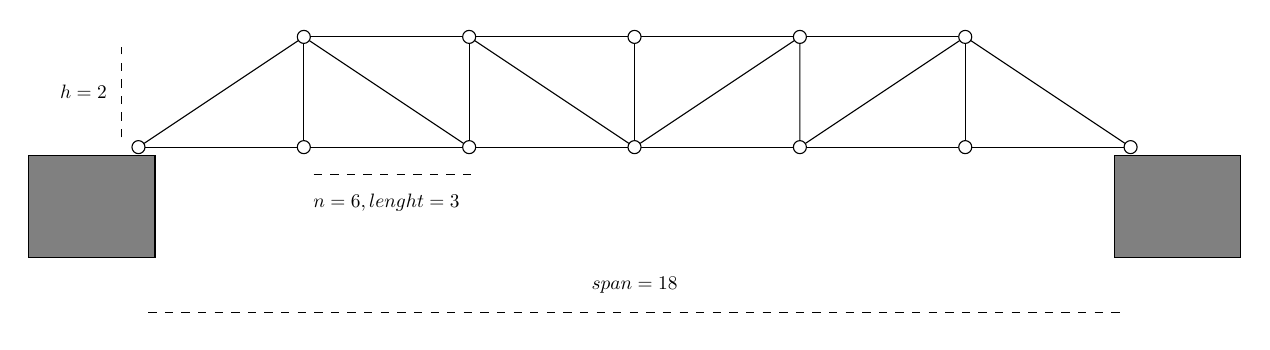
\begin{tikzpicture}[scale = 0.7]

    \tikzset{nodestyle/.style={draw,shape=circle,scale=0.5}}
    \node[nodestyle] (p1) at ( 0, 0) {}; 
    \node[nodestyle] (p2) at ( 3, 0) {};
    \node[nodestyle] (p3) at ( 6, 0) {};
    \node[nodestyle] (p4) at ( 9, 0) {};
    \node[nodestyle] (p5) at ( 12, 0) {};
    \node[nodestyle] (p6) at ( 15, 0) {};
    \node[nodestyle] (p7) at ( 18, 0) {};

    \node[nodestyle] (p8) at ( 3, 2) {};
    \node[nodestyle] (p9) at ( 6, 2) {};
    \node[nodestyle] (p10) at ( 9, 2) {};
    \node[nodestyle] (p11) at ( 12, 2) {};
    \node[nodestyle] (p12) at ( 15, 2) {};

    \begin{scope}[every path/.style={-}]
        \draw (p1) -- (p2);
        \draw (p2) -- (p3); 
        \draw (p3) -- (p4);
        \draw (p4) -- (p5);
        \draw (p5) -- (p6);
        \draw (p6) -- (p7);

        \draw (p8) -- (p9);
        \draw (p9) -- (p10);
        \draw (p10) -- (p11);
        \draw (p11) -- (p12);

        \draw (p1) -- (p8);
        \draw (p12) -- (p7);

        \draw (p2) -- (p8);
        \draw (p3) -- (p9);
        \draw (p4) -- (p10);
        \draw (p5) -- (p11);
        \draw (p6) -- (p12);

        \draw (p8) -- (p3);
        \draw (p9) -- (p4);
        \draw (p4) -- (p11);
        \draw (p5) -- (p12);
    \end{scope}  

        \draw[fill=gray] (0.3,-0.15) rectangle (-2,-2);
        \draw[fill=gray] (17.7,-0.15) rectangle (20,-2);

        % Nodos artificiales.
        \node (a1) at ( 0, -3) {};
        \node (a2) at ( 18, -3) {};
        \node (a3) at ( -0.3, 0) {};
        \node (a4) at ( -0.3, 2) {};
        \node (a5) at ( 3, -0.5) {};
        \node (a6) at ( 6.3, -0.5) {};
        \node[scale=0.7] (l1) at ( 9, -2.5) {$span = 18$};
        \node[scale=0.7] (l2) at ( -1, 1) {$h = 2$};
        \node[scale=0.7] (l2) at ( 4.5, -1) {$n = 6, lenght = 3$};
        
        \begin{scope}[every path/.style={-}]
            \draw[dashed] (a1) -- (a2) ;
            \draw[dashed] (a3) -- (a4) ;
            \draw[dashed] (a5) -- (a6) ;
        \end{scope}
        
\end{tikzpicture}
\caption{Ejemplo estructura en 2D}
\label{fig:structex}
\end{center}
\end{figure}

\noindent La estructura mostrada como ejemplo cuenta un $span$ de 18 metros, una altura $h = 2m$ y 6 secciones. Dentro
del presente trabajo, analizaremos puentes que tienen exactamente el patr\'on descripto en el ejemplo en t\'erminos
de sim\'etr\'ia y conformaci\'on de la estructura, pero con diferentes valores de $span$, $h$ y $n$.

Para que la estructura del puente pueda ser utilizada, debe soportar una carga total (conocida) que se distribuye entre 
las juntas internas inferiores del puente. Este hecho afecta a toda la estructura del puente y por lo tanto los links
que conforman la misma deben ser lo suficientemente resistentes para mantener estable la estructura. El objetivo del
trabajo es realizar este an\'alisis para distintos tipos de estructuras.

\textbf{El problema}

Dado un puente Pratt Truss con $n$ secciones, la estructura cuenta con $4n-3$ links y $2n$ juntas. A su vez, para cada
uno de las $n-1$ juntas internas inferiores suponemos que se aplica una carga $c_i$, $i = 1,\dots,n-1$. Llamamos $F_j$ a
la fuerza ejercida sobre el link $j$, $j = 1,\dots,4n-3$, dada una numeraci\'on para los links. Nuestro objetivo es
calcular la compresi\'on ($F_i < 0$) o tensi\'on ($F_i > 0$) a cada link de la estructura una vez que las fuerzas se
aplican a la estructura. 

Adem\'as de las fuerzas para cada link, consideramos tambi\'en otras tres fuerzas soporte que se aplican sobre los extremos
inferiores de la estructura. Las llamaremos $v_0, v_1$ y $h_0$. La Figura \ref{fig:structload} muestra como se aplican
las definiciones a la estructura.

\begin{figure}[!ht]
\begin{center}
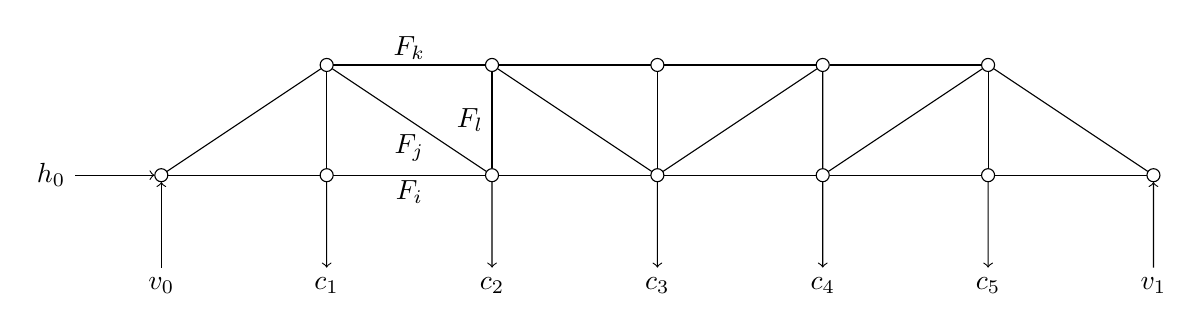
\begin{tikzpicture}[scale = 0.7]

    \tikzset{nodestyle/.style={draw,shape=circle,scale=0.5}}
    \node[nodestyle] (p1) at ( 0, 0) {}; 
    \node[nodestyle] (p2) at ( 3, 0) {};
    \node[nodestyle] (p3) at ( 6, 0) {};
    \node[nodestyle] (p4) at ( 9, 0) {};
    \node[nodestyle] (p5) at ( 12, 0) {};
    \node[nodestyle] (p6) at ( 15, 0) {};
    \node[nodestyle] (p7) at ( 18, 0) {};

    \node[nodestyle] (p8) at ( 3, 2) {};
    \node[nodestyle] (p9) at ( 6, 2) {};
    \node[nodestyle] (p10) at ( 9, 2) {};
    \node[nodestyle] (p11) at ( 12, 2) {};
    \node[nodestyle] (p12) at ( 15, 2) {};

    \begin{scope}[every path/.style={-}]
        \draw (p1) -- (p2);
        \draw (p2) -- (p3); 
        \draw (p3) -- (p4);
        \draw (p4) -- (p5);
        \draw (p5) -- (p6);
        \draw (p6) -- (p7);

        \draw (p8) -- (p9);
        \draw (p9) -- (p10);
        \draw (p10) -- (p11);
        \draw (p11) -- (p12);

        \draw (p1) -- (p8);
        \draw (p12) -- (p7);

        \draw (p2) -- (p8);
        \draw (p3) -- (p9);
        \draw (p4) -- (p10);
        \draw (p5) -- (p11);
        \draw (p6) -- (p12);

        \draw (p8) -- (p3);
        \draw (p9) -- (p4);
        \draw (p4) -- (p11);
        \draw (p5) -- (p12);
    \end{scope}  

    
    \node (v0) at ( 0, -2) {$v_0$};
    \node (v1) at ( 18, -2) {$v_1$};
    \node (h0) at ( -2, 0) {$h_0$};
    \node (c1) at ( 3, -2) {$c_1$};
    \node (c2) at ( 6, -2) {$c_2$};
    \node (c3) at ( 9, -2) {$c_3$};
    \node (c4) at ( 12, -2) {$c_4$};
    \node (c5) at ( 15, -2) {$c_5$};

    \node (fi) at ( 4.5, -0.3) {$F_i$};
    \node (fj) at ( 4.5, 0.5) {$F_j$};
    \node (fj) at ( 4.5, 2.3) {$F_k$};
    \node (fj) at ( 5.6, 1) {$F_l$};

    %\begin{scope}[every path/.style={-}]
        \draw[->] (v0) -- (p1);
        \draw[->] (v1) -- (p7);
        \draw[->] (h0) -- (p1);
        \draw[->] (p2) -- (c1);
        \draw[->] (p3) -- (c2);
        \draw[->] (p4) -- (c3);
        \draw[->] (p5) -- (c4);
        \draw[->] (p6) -- (c5);
    %\end{scope}

        % Nodos artificiales.
         
\end{tikzpicture}
\caption{Fuerzas aplicadas sobre la estructura}
\label{fig:structload}
\end{center}
\end{figure}

Para que la estructura se encuentre en equilibrio (es decir, que no se este moviendo) se establece que la fuerza total
que se aplica sobre el mismo es cero.  Luego, para
cada junta, se tienen que cumplir que la suma de las fuerzas que act\'uan horizontalmente sea cero, y an\'alogamente que
la suma de las fuerzas verticales tambi\'en sea nula, obteniendo dos ecuaciones por cada junta presente en la
estructura. Con el objetivo de simplificar el an\'alisis, en este caso suponemos que la carga se aplica 
solamente sobre las juntas, que los links son perfectamente rectos y que el peso de la estructura es cero.

La Figura \ref{fig:jointforce} muestra el diagrama de fuerzas sobre una junta en particular. Es importante destacar que
la fuerza correspondiente al link $j$, $F_j$, debe descomponerse en sus componentes vertical y horizontal. Luego, las
ecuaciones de equilibrio para la junta son:

\begin{eqnarray}
F_i + F_j \cos(\theta) - F_k & = & 0 ~~~~~ \textrm{(Horizontal)} \\
F_j \sin(\theta) + F_l + c_2 & = & 0 ~~~~~ \textrm{(Vertical)}
\end{eqnarray}

Planteando estas ecuaciones para cada junta, obtenemos un total de $4n$ ecuaciones y $4n$ inc\'ognitas ($4n-3$
correspondientes a las variables $F_i$ y $v_0$, $v_1$ y $h_0$). Un primer objetivo del trabajo consiste resolver este
sistema de ecuaciones utilizando un m\'etodo directo.

\begin{figure}[!ht]
\begin{center}
\begin{tikzpicture}[]

    \tikzset{nodestyle/.style={draw,shape=circle}}
    \node (p2) at ( 3, 0) {};
    \node[nodestyle] (p3) at ( 6, 0) {};
    \node (p4) at ( 9, 0) {};

    \node (p8) at ( 3, 3) {};
    \node (p9) at ( 6, 3) {};

    \begin{scope}[every path/.style={->,thick}]
        \draw (p2) -- (p3); 
        \draw (p4) -- (p3);

        \draw (p9) -- (p3);
        \draw (p8) -- (p3);

    \end{scope}  

    
    \node (c2) at ( 6, -2) {$c_2$};
    \node (ang) at ( 5.3, 0.3) {$\theta$};

    \node (fi) at ( 4, -0.3) {$F_i$};
    \node (fj) at ( 4, 1) {$F_j$};
    \node (fl) at ( 5.6, 2.2) {$F_l$};
    \node (fk) at ( 8, -0.3) {$F_k$};

    %\begin{scope}[every path/.style={-}]
        \draw[->,thick] (p3) -- (c2);
    %\end{scope}
%\draw (5,0) arc (45:0:-1);
\draw[domain=135:180] plot ({6+cos(\x)}, {sin(\x)});
        % Nodos artificiales.
\end{tikzpicture}
\caption{Fuerzas aplicadas sobre una junta}
\label{fig:jointforce}
\end{center}
\end{figure}

Adem\'as de la informaci\'on sobre la estructura, se tiene como dato un valor m\'aximo de la fuerza que puede resistir cualquier
link de la estructura, bas\'andose en los materiales disponibles en el mercado. Se denomina a este valor $fmax$. Una vez
calculadas las fuerzas ejercidas sobre cada link, si el valor absoluto de alguna de ellas excediera $fmax$, entonces la
estructura no cumple con las condiciones m\'inimas de seguridad y podr\'ia colapsar. Sin embargo, existe la posibilidad
de intercalar pilares de concreto intermedios (debajo de las juntas internas inferiores) para contrarrestrar este
efecto, particionando la estructura original en sub-estructuras. Es importante mencionar que las sub-estructuras deben
cumplir con las restricciones de la estructura original (por ejemplo, tener un n\'umero par de secciones) y, por lo
tanto, se puede realizar exactamente el mismo an\'alisis sobre estructuras m\'as peque\~nas. 
Como contraparte, cada uno de estos pilares es muy costoso y se busca minimizar la utilizaci\'on de los mismos. Las
figura \ref{fig:partexorig} y \ref{fig:partexres} muestra un ejemplo de una partici\'on posible.

\begin{figure}[!ht]
\begin{center}
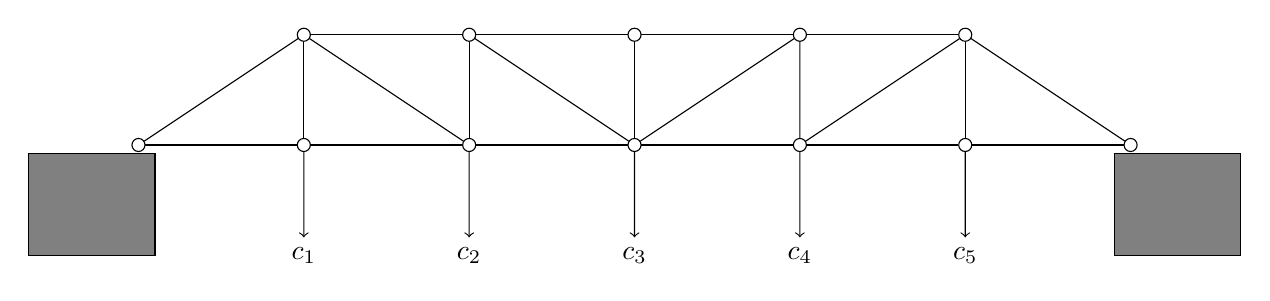
\begin{tikzpicture}[scale = 0.7]

    \tikzset{nodestyle/.style={draw,shape=circle,scale=0.5}}
    \node[nodestyle] (p1) at ( 0, 0) {}; 
    \node[nodestyle] (p2) at ( 3, 0) {};
    \node[nodestyle] (p3) at ( 6, 0) {};
    \node[nodestyle] (p4) at ( 9, 0) {};
    \node[nodestyle] (p5) at ( 12, 0) {};
    \node[nodestyle] (p6) at ( 15, 0) {};
    \node[nodestyle] (p7) at ( 18, 0) {};

    \node[nodestyle] (p8) at ( 3, 2) {};
    \node[nodestyle] (p9) at ( 6, 2) {};
    \node[nodestyle] (p10) at ( 9, 2) {};
    \node[nodestyle] (p11) at ( 12, 2) {};
    \node[nodestyle] (p12) at ( 15, 2) {};

    \begin{scope}[every path/.style={-}]
        \draw (p1) -- (p2);
        \draw (p2) -- (p3); 
        \draw (p3) -- (p4);
        \draw (p4) -- (p5);
        \draw (p5) -- (p6);
        \draw (p6) -- (p7);

        \draw (p8) -- (p9);
        \draw (p9) -- (p10);
        \draw (p10) -- (p11);
        \draw (p11) -- (p12);

        \draw (p1) -- (p8);
        \draw (p12) -- (p7);

        \draw (p2) -- (p8);
        \draw (p3) -- (p9);
        \draw (p4) -- (p10);
        \draw (p5) -- (p11);
        \draw (p6) -- (p12);

        \draw (p8) -- (p3);
        \draw (p9) -- (p4);
        \draw (p4) -- (p11);
        \draw (p5) -- (p12);
    \end{scope}  

        \draw[fill=gray] (0.3,-0.15) rectangle (-2,-2);
        \draw[fill=gray] (17.7,-0.15) rectangle (20,-2);

    \node (c1) at ( 3, -2) {$c_1$};
    \node (c2) at ( 6, -2) {$c_2$};
    \node (c3) at ( 9, -2) {$c_3$};
    \node (c4) at ( 12, -2) {$c_4$};
    \node (c5) at ( 15, -2) {$c_5$};
    \draw[->] (p2) -- (c1);
    \draw[->] (p3) -- (c2);
    \draw[->] (p4) -- (c3);
    \draw[->] (p5) -- (c4);
    \draw[->] (p6) -- (c5);


\end{tikzpicture}
\caption{Estructura original}
\label{fig:partexorig}
\end{center}
\end{figure}


\begin{figure}[!ht]
\begin{center}
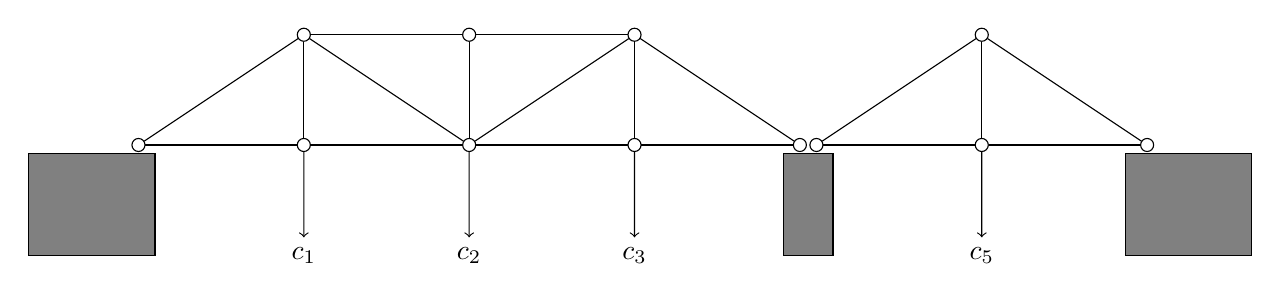
\begin{tikzpicture}[scale = 0.7]

    \tikzset{nodestyle/.style={draw,shape=circle,scale=0.5}}
    \node[nodestyle] (p1) at ( 0, 0) {}; 
    \node[nodestyle] (p2) at ( 3, 0) {};
    \node[nodestyle] (p3) at ( 6, 0) {};
    \node[nodestyle] (p4) at ( 9, 0) {};
    \node[nodestyle] (p5) at ( 12, 0) {};
    \node[nodestyle] (p8) at ( 3, 2) {};
    \node[nodestyle] (p9) at ( 6, 2) {};
    \node[nodestyle] (p10) at ( 9, 2) {};

    \begin{scope}[every path/.style={-}]
        \draw (p1) -- (p2);
        \draw (p2) -- (p3); 
        \draw (p3) -- (p4);
        \draw (p4) -- (p5);
        \draw (p8) -- (p9);
        \draw (p9) -- (p10);
        \draw (p1) -- (p8);
        \draw (p2) -- (p8);
        \draw (p3) -- (p9);
        \draw (p4) -- (p10);
        \draw (p8) -- (p3);
        \draw (p3) -- (p10);
        \draw (p10) -- (p5);
    \end{scope}  

        \draw[fill=gray] (0.3,-0.15) rectangle (-2,-2);
        \draw[fill=gray] (11.7,-0.15) rectangle (12.6,-2);

     % Segundo puente

    \node[nodestyle] (q1) at ( 12.3, 0) {};
    \node[nodestyle] (q2) at ( 15.3, 0) {};
    \node[nodestyle] (q3) at ( 18.3, 0) {};
    \node[nodestyle] (q4) at ( 15.3, 2) {};

    \begin{scope}[every path/.style={-}]
        \draw (q1) -- (q2);
        \draw (q2) -- (q3);
        \draw (q1) -- (q4);
        \draw (q2) -- (q4);
        \draw (q4) -- (q3);
    \end{scope}


    \draw[fill=gray] (17.9,-0.15) rectangle (20.2,-2);

    \node (c1) at ( 3, -2) {$c_1$};
    \node (c2) at ( 6, -2) {$c_2$};
    \node (c3) at ( 9, -2) {$c_3$};
    \node (c5) at ( 15.3, -2) {$c_5$};
    \draw[->] (p2) -- (c1);
    \draw[->] (p3) -- (c2);
    \draw[->] (p4) -- (c3);
    \draw[->] (q2) -- (c5);

\end{tikzpicture}
\caption{Estructura particionada.}
\label{fig:partexres}
\end{center}
\end{figure}

El costo total del puente, que llamaremos $c_{\textrm{total}}$, se calcula en base a los costos parciales de cada sub-estructura
sumado al costo de construcci\'on de los pilares. Dada una sub-estructura $e$ (es decir, un punte Pratt Truss sin pilares
en las juntas internas inferiores) el costo parcial, $cp_e$, ser\'a proporcional a la m\'axima fuerza ejercida y la longitud del
mismo. Luego, $cp_e$ se computa como 
\begin{displaymath}
cp_e = \max_{\substack{i \textrm{ link}\\ i\in e}}|F_i|\Bigg(\sum_{\substack{i \textrm{ link}\\ i\in e}} l_i\Bigg),
\end{displaymath}
donde $l_i$ es la longitud de link $i$ perteneciente a la estructura $e$. Adem\'as, se cuenta con un costo fijo de
construcci\'on de pilares, que llamaremos $C$. Sean $e_1,\dots,e_k$ las sub-estructuras seguras (es decir, ninguna de
las fuerzas aplicadas sobre sus respectivos links excede $fmax$), el costo total del puente se calcula como
\begin{displaymath}
c_{\textrm{total}} = \sum_{i = 1}^k cp_{e_i} + (k-1)C.
\end{displaymath}

El segundo objetivo del trabajo es, mediante esta t\'ecnica de inserci\'on de pilares de concreto, obtener una
estructura que sea considerada segura para su utilizaci\'on buscando minimizar el costo total de la misma.

\textbf{Enunciado}

El trabajo pr\'actico consiste en proveer una herramienta que, dados el $span$, $h$, y $n$, formule el sistema de
ecuaciones provisto por las condiciones de equilibrio y calcule la fuerza ejercida sobre cada uno de los links de la
estructura en dos dimensiones de un puente Pratt Truss.

Los requisitos m\'inimos a cumplir son los siguientes:

\begin{itemize}
\item Formular el sistema lineal de forma tal que la matriz resultante cumpla la propiedad de ser banda $p,q$, donde
estos valores deben estar acotados por una constante. 

\item Implementar el m\'etodo de Eliminaci\'on Gaussiana con pivoteo parcial. Para ello, considerar que al aplicar este
m\'etodo
sobre una matriz banda $p,q$, en el peor caso la matriz resultante tendr\'a bandas $p,q+p$. Demostrar este resultado, y
utilizarlo para almacenar el sistema de forma eficiente en t\'erminos de memoria utilizada.

\item Realizar experimentos computacionales comparativos analizando como evoluciona el valor absoluto de la maxima fuerza ejercida
sobre alguno de los links de la estructura en funci\'on del $span$ (fijando $h$ y los valores de $c_i$) y de los
valores de $c_i$ (fijando el $span$ y $h$) para distintos valores de $n$, adem\'as de cualquier otro experimento que
considere pertinente.

\item Bas\'andose en el an\'alisis anterior, proponer un m\'etodo heur\'istico que permita simular el agregado de
pilares de concreto mediante la partici\'on de la estructura original en sub-estructuras, de forma tal que el puente 
sea seguro, buscando minimizar el costo total de construcci\'on del puente.
\end{itemize}

\textbf{Competencia}

La c\'atedra realizar\'a una competencia donde se analizar\'an los resultados obtenidos por los distintos grupos sobre
distintas instancias del problema donde la estructura original no es segura. El programa provisto por cada grupo ser\'a
analizado en la competencia y se armar\'a un ranking en funci\'on de los resultados obtenidos. El primer puesto ser\'a
reconocido con el premio \emph{Listos para usar casco} y tambi\'en habra una distinci\'on para el segundo puesto. 
Las condiciones de la competencia ser\'an publicadas el Lunes 23 de Septiembre de 2013.

\underline{Aclaraci\'on:} La nota de los trabajos es independiente de los resultados de esta competencia y depende \'unicamente del
trabajo realizado.

\vskip 15pt

\hrule

\vskip 11pt


{\bf \underline{Fechas de entrega}}
\begin{itemize}
 \item \emph{Formato Electr\'onico:} Domingo 6 de Octubre de 2013, hasta las 23:59 hs, enviando el trabajo (informe +
 c\'odigo) a la direcci\'on \verb+metnum.lab@gmail.com+. El subject del email debe comenzar con el texto \verb+[TP2]+
 seguido de la lista de apellidos  de los integrantes del grupo.
 \item \emph{Formato f\'isico:} Lunes 7 de Octubre de 2013, de 17 a 18 hs.
\end{itemize}

\noindent \textbf{Importante:} El horario es estricto. Los correos recibidos despu\'es de la hora indicada ser\'an considerados re-entrega.  

\begin{comment}
\newpage

\textbf{Resoluci\'on}

El primer item importante de la resolucion del sistema es el modelado. Para eso, tienen primero que analizar como se
descomponen las fuerzas correspondientes a links diagonales depndiendo de la ecuaci\'on en cuesti\'on. Una vez que
tienen eso, deben decidir como numerar los links/juntas para que el armado del sistema les quede banda. Una numeraci\'on
correlativa de izquierda a derecha deberia llevarlos a un sistema con una estructura similar al que se muestra en la
Figura \ref{fig:matrixspy}, que corresponde a un caso en particular. Los puntos azules son elementos distintos de cero
de la matriz que estan fuera de la diagonal, los rojos aquellos que estan en la diagonal, y finalmente los verdes
posiciones de la diagonal de la matriz que son cero. 

\begin{figure}[!ht]
\begin{center}
\includegraphics[scale=0.5]{matrixspy.jpg}
\caption{Estructura de la matriz.}
\label{fig:matrixspy}
\end{center}
\end{figure}

Respecto de la resoluci\'on del sistema, se sugiere utilizar Eliminaci\'on Gaussiana con pivoteo parcial ya que (despues
de pensarlo un rato) no se me ocurrio una forma de garantizar que esto no es necesario. Es posible que exista alg\'un
ordenamiento que, combinado con alg\'un otro resultado, permita concluir que no es necesario pivotear. En este caso, si
efectivamente alg\'un grupo puede justificar esto, la idea ser\'a tomar como v\'alido que utilicen directamente
Eliminaci\'on Gaussiana standard. 

En caso de utilizar Eliminaci\'on Gaussiana con pivoteo parcial, dado que el sistema es banda, se les pide probar un
resultado relativamente simple para que lo utilicen. La demostraci\'on no es dificil y (creo) les va a ayudar a entender
con m\'as detalle el sistema.

Una vez que resuelven el sistema, la soluci\'on se interpreta de forma similar a lo que muestra la Figura
\ref{fig:solutionexample}. Este graficador no lo implementamos nosotros y no se lo vamos a proveer, ya que el mismo
establece una numeraci\'on para las variables y por lo tanto le quitar\'ia gracia al modelado del problema.

\begin{figure}[!ht]
\begin{center}
\includegraphics[scale=0.4]{res1.jpg}
\caption{Ejemplo de soluci\'on.}
\label{fig:solutionexample}
\end{center}
\end{figure}

El siguiente punto es realizar un par de experimentos, como para que computacionalmente eval\'uen como evolucionan las
fuerzas aplicadas sobre la estructura dependiendo de algunos par\'ametros de entrada. Las figuras \ref{fig:fvsspan} y
\ref{fig:fvsforce} muestran que pasa con la fuerza m\'axima aplicada sobre los links en funci\'on del $span$ y la fuerza
total aplicada para estructuras con distinta cantidad de secciones. Parte del objetivo de este an\'alisis esta
relacionada con la \'ultima etapa del TP: la competencia.

La idea detr\'as de la competencia es que sirva como motivaci\'on para prestar atenci\'on a la implementaci\'on del
m\'etodo de resoluci\'on de sistemas y la realizaci\'on de experimentos. B\'asicamente, una vez que tienen las rutinas
para resolver el sistema, la idea es que las utilicen de alguna forma para tomar decisiones respecto al armado del
puente teniendo en cuenta una restricci\'on de seguridad (limite sobre la fuerza aplicada a los links de la estructura).
El objetivo de esta etapa es que el TP no sea solamente resolver el sistema, si no tambi\'en tomar la soluci\'on,
interpretarla y utilizar la informaci\'on provista por la misma para tomar una decisi\'on.
Esta etapa es m\'as l\'udica que real, y la cantidad de secciones se deja fija para que no puedan especular con aumentar
el n\'umero de las mismas indiscriminadamente y bajar la fuerza m\'axima aplicada. Por otro lado, el agregado de pilares
de concreto va a tener un costo muy alto de forma tal que nunca sea conveniente agregarlos, a menos que la condici\'on
de seguridad no se cumpla. Ademas, dado que cada sub-estructura tiene tambien asociado un costo que depende de la
m\'axima fuerza ejercida sobre alguno de sus links y la longitud de la misma, tampoco da lo mismo poner los pilares en
cualquier lugar. En definitiva, la idea es que propongan algo heuristico donde, dada las condiciones que deben cumplir
las subestructura, reacomodar algunos parametros de entrada y llamar a la rutina general para calcular las fuerzas. Esto
no deber\'ia agregar demasiada complejidad para una soluci\'on simple, como por ejemplo algo iterativo que resuelve el
sistema completo, se analiza la seguridad, se decide poner un pilar en alg\'un punto, y luego se aplica el mismo
razonamiento sobre las sub-estructuras definidas.

En funci\'on de la evaluaci\'on de la competencia, se les dar\'a a los alumnos un set de instacias de prueba donde
puedan testear la estrategia definida. Luego, el d\'ia que devolvamos los TPs, haremos en clase una competencia sobre
instacias desconocidas para ellos y los ordenaremos en funci\'on de los resultados. Las bases de la competencia las
vamos a presentar el Lunes siguiente al de la presentaci\'on del TP. Para el primer puesto el premio es un casco de
construcci\'on usado (como si fuera una camiseta transpirada de un jugador de futbol) y estamos pensando cual va a ser 
el premio para el segundo puesto.

\begin{figure}[!ht]
\begin{center}
\includegraphics[scale=0.5]{maxfvsspan.jpg}
\caption{$\max F_i$ vs. $span$.}
\label{fig:fvsspan}
\end{center}
\end{figure}

\begin{figure}[!ht]
\begin{center}
\includegraphics[scale=0.5]{maxfvsforce.jpg}
\caption{$\max F_i$ vs. carga total.}
\label{fig:fvsforce}
\end{center}
\end{figure}
\end{comment}
